\documentclass[border=10pt]{standalone}

\usepackage{tikz}
\usetikzlibrary{arrows.meta,arrows,decorations.pathmorphing,backgrounds,positioning,fit,petri,calc,shapes.geometric,scopes,fit,spy,chains}
\usepackage{pgfplots}
\pgfplotsset{,compat=1.11}
\tikzset{/pgf/number format/1000 sep={\,}}

\usepackage{fontawesome5}
\renewcommand{\familydefault}{\sfdefault}
\usepackage{helvet}
\begin{document}

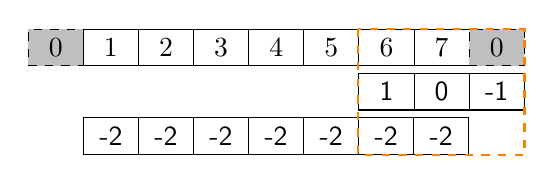
\begin{tikzpicture}[start chain=1 going right,%
        start chain=2 going right,%
        node distance=-0.15mm, %
        minimum width=.7cm,
        auto]

        % %% first line
      %   \node [dashed, fill=lightgray,draw] (ghost_li0_1) {$0$};
      %   \foreach \a in {1,...,7} {
      %     \node [draw,name=xfield_li0_\a] at($(ghost_li0_1)+(\a*.7,0)$) {$\a$};
      %   }
      %   \node [dashed, fill=lightgray,draw] (ghost_li0_2) at($(xfield_li0_7)+(.7,0)$) {$0$};
      %   \node [draw] (krnl_li0_0) at($(ghost_li0_1)+(0,-24pt)$) {1};
      %   \node [draw] (krnl_li0_1) at($(krnl_li0_0)+(.7,0)$) {0};
      %   \node [draw] (krnl_li0_2) at($(krnl_li0_1)+(0.7,0)$) {-1};

      %   \node [draw,on chain=1] (res_li0_1) at($(krnl_li0_1)+(0,-24pt)$) {$-2$};
      %   \foreach \a in {2,...,7} {
      %     \a, \node [draw,name=res_li0_\a,on chain=1] {0};
      %   }
      %   \draw[thick,dashed,color=orange]  ($(ghost_li0_1.north west)$) rectangle ($(res_li0_2.south east)$);
      %   \node [color=orange] (cdot_li0_0) at($(krnl_li0_1)!.5!(xfield_li0_1)$) {$\ast$};
      %   \node [color=orange] (equl_li0_0) at($(krnl_li0_1)!.5!(res_li0_1)$) {$=$};

      %   %% second line
      %   % \uncover<2->{
      % %   \node [dashed, fill=lightgray,draw] (ghost_li1_1) at($(ghost_li0_1)+(0,-2.75cm)$) {$0$};
      % %   \foreach \a in {1,...,7} {
      % %     \node [draw,name=xfield_li1_\a] at($(ghost_li1_1)+(\a*.7,0)$) {$\a$};
      % %   }
      % %   \node [dashed, fill=lightgray,draw] (ghost_li1_2) at($(xfield_li1_7)+(.7,0)$) {$0$};
      % %   \node [draw] (krnl_li1_0) at($(xfield_li1_1)+(0,-16pt)$) {1};
      % %   \node [draw] (krnl_li1_1) at($(krnl_li1_0)+(.7,0)$) {0};
      % %   \node [draw] (krnl_li1_2) at($(krnl_li1_1)+(0.7,0)$) {-1};

      % %   \node [draw,on chain=1] (res_li1_2) at($(krnl_li1_1)+(-0.35,-16pt)$) {-2};
      % %   \node [draw] (res_li1_1) at($(res_li1_2)+(-.7,0)$) {-2};
      % %   \foreach \a in {3,...,7} {
      % %     \a, \node [draw,name=res_li1_\a,on chain=1] {0};
      % %   }
      % %   \draw[thick,dashed,color=orange]  ($(xfield_li1_1.north west)$) rectangle ($(res_li1_3.south east)$);
      % %   }
        %% third line
        
        \node [dashed, fill=lightgray,draw] (ghost_li2_1) at(0,0) {$0$};
        \foreach \a in {1,...,7} {
          \node [draw,name=xfield_li2_\a] at($(ghost_li2_1)+(\a*.7,0)$) {$\a$};
        }
        \node [dashed, fill=lightgray,draw] (ghost_li2_2) at($(xfield_li2_7)+(.7,0)$) {$0$};
        \node [draw] (krnl_li2_0) at($(xfield_li2_6)+(0,-16pt)$) {1};
        \node [draw] (krnl_li2_1) at($(krnl_li2_0)+(.7,0)$) {0};
        \node [draw] (krnl_li2_2) at($(krnl_li2_1)+(0.7,0)$) {-1};

        \node [draw,on chain=1] (res_li2_1) at($(xfield_li2_1)+(0.,-32pt)$) {-2};
        % \node [draw] (res_li2_2) at($(res_li2_3)+(-.7,0)$) {-2};
        % \node [draw] (res_li2_1) at($(res_li2_2)+(-.7,0)$) {-2};
        \foreach \a in {2,...,7} {
          \a, \node [draw,name=res_li2_\a,on chain=1] {-2};
        }
        \draw[thick,dashed,color=orange]  ($(xfield_li2_6.north west)$) rectangle ($(res_li2_7.south east)+(.7,0)$);
      
      \end{tikzpicture}
\end{document}
